% https://tex.stackexchange.com/questions/144577/remove-chapter-number-from-bibliography

\documentclass[
a4paper, 
11pt, 
ngerman,
listof=totoc,
%oneside,
%bibliography=totoc,
bibliography=totocnumbered,
abstracton
]{scrreprt}

\usepackage[T1]{fontenc}
\usepackage[utf8]{inputenc}
\usepackage[ngerman]{babel}
\usepackage{graphicx}
\usepackage{lipsum}
\usepackage{csquotes}
\usepackage[onehalfspacing]{setspace}
\usepackage{scrlayer-scrpage}
\usepackage{float}
\usepackage{mhchem}
\usepackage{siunitx}
\chead*{\pagemark}
\cofoot*{}

%\usepackage{lineno}
%\usepackage{layout}
%
%\makeatletter
%\renewcommand*{\lay@value}[2]{%
%	\strip@pt\dimexpr0.351459\dimexpr\csname#2\endcsname\relax\relax mm%
%}
%\makeatother

%\usepackage[showframe]{geometry}
%
%\geometry{
%	top = 2.5cm,
%	bottom = 2.5cm,
%	left = 3.5cm,
%	right = 2.5cm
%	}

\usepackage[
backend=biber,
style=authoryear-ibid,
%sorting=ynt
]{biblatex}
\addbibresource{gravitropismus-bibliography.bib}

\title{Untersuchung von Gravitropismus bei \emph{Lepidium sativum} mit einem selbstgebauten Klinostat unter Zimmerbedingungen}

\subtitle{W-Seminararbeit im Fach Biologie am Luitpold-Gymnasium München}

\author{Alexandra Smirnova}


\begin{document}
	
\begingroup
\renewcommand*{\chapterpagestyle}{empty}
\pagestyle{empty}
\maketitle
\tableofcontents
\clearpage
\endgroup
	
\renewcommand\abstractname{Abstract}
\begin{abstract}

	
\end{abstract}

% \let\raggedsection\centering
% \section*{\abstractname}
% Dies ist die Zusammenfassung auf Deutsch.

\chapter{Gravitropismus als wichtige Pflanzeneigenschaft}

Viele Pflanzen sind an die Erde festgebundene Organismen, die seit ihrer Keimung ihr ganzes Leben an einem Ort verbringen. Dabei werden die Pflanzen durch Wurzeln an die Erde verankert. 

Gravitropismus wurde vor zweihundert Jahren anerkannt (Knight, 1806). Experimente mit verschiedenen Pflanzen wie zum Beispiel der \emph{arabidopsis}

-aktives Forschungsthema (aktuelle Publikationen, die sich damit befassen) kosmos etc.
-meine Arbeit




%Mit Anführungszeichen: {\glqq Term mit\grqq} bla adsfa asf. asdfasdf



\chapter{Fachliche Analyse der Thematik Gravitropismus}

In der vorliegenden Arbeit wird die Theorie des Gravitropismus kurz geklärt und dann im experimentellen Teil nachgewiesen. Zuerst werden für den Gravitropismus grundlegende Begriffe aus der Botanik geklärt, um die Reizaufnahme, die Signaltransduktion und das darauf folgende differenzielles Wachstum besser verstehen zu können.  



\section{Für den Gravitropismus grundlegende Begriffe aus der Botanik}

\subsection{Morphologie der Pflanze}

\begin{figure}[H]
	\centering 
	\includegraphics[width = 0.4\linewidth]{bilder/Pflanzenaufbau.png}
	\caption{Pflanzenaufbau  \label{Pflanzenaufbau}}
\end{figure} 

\subsection{Arten des Gravitropismus}

Beim Gravitropismus, auch genannt Geotropismus, werden drei Bewegungsarten unterschieden: \emph{Positiv gravitrop},  \emph{negativ gravitrop} und  \emph{transversalgravitrop}.
Positiv gravitrop bedeutet, dass das Wachstum der Organe, wie zum Beispiel Wurzeln, Rhizoide (wurzelähnliche Strukturen), Moose oder Farnprothallien, zur Schwerkraftquelle hin (nach unten zur Erdmitte) erfolgt.
Negativ gravitrope Organe dagegen, wie Sprossen, Sporangienträger der Schimmelpilze der Gattung \emph{Mucor} oder Fruchtkörper mancher Pilze wachsen von der Schwerkraftquelle weg (nach oben).

Diese zwei Wachstumsrichtungen werden auch als \emph{Orthogravitropismus} bezeichnet, da sie beide parallel zur Schwerkraft wachsen \parencite[546]{Jacob}.
Seitenwurzeln der ersten Ordnung (Nebenwurzeln, die von der Hauptwurzel entspringen) und zahlreiche Seitenzweige sowie Blätter wachsen \emph{ transversalgravitrop}: entweder horizontal oder quer nach unten in einem bestimmten Winkel \parencite[449]{Strasburger}. 

\begin{figure}[H]
\centering 
 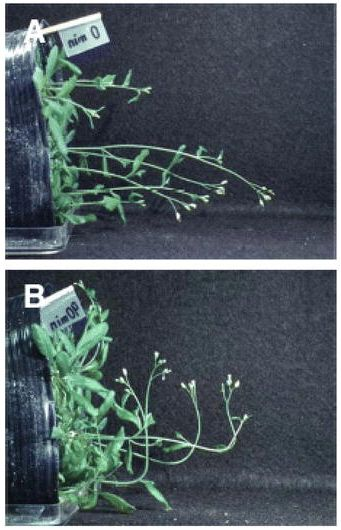
\includegraphics[width = 0.3\linewidth]{bilder/gravitrop_reagierende_Pflanze.jpg}
 \caption{Gravitrop reagirende \emph{Arabidopsis thaliana} \label{gravitrop_reagierende_Pflanze}}
\end{figure} 
 
Legt man eine Pflanze quer, so werden sich Wurzeln und Spross krümmen, bis sie senkrecht stehen und wieder positiv bzw. negativ gravitrop wachsen
\parencite[528]{Luettge}.






\section{Reizaufnahme}

Damit eine gravitrope Krümmung entstehen kann, werden zuvor Reize durch \emph{Statolithen}, schwere Körperteilchen oder Organelle in bestimmten Zellen des Sprosses, der \emph{Koleoptil}-, und der Wurzelspitzen aufgenommen. Es handelt sich dabei meist um \emph{Amyloplasten}, die aus Stärke bestehen \parencite[530]{Luettge}.

\begin{figure}[H]
	\centering 
	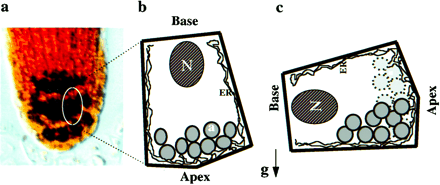
\includegraphics[width = 0.4\linewidth]{bilder/Statolithen2.png}
	\caption{Statolithen \label{Statolithen}}
\end{figure} 

Entscheidend ist der Stärkegehalt  der Amyloplasten, denn ohne ihn geht die gravitrope Reaktionfähigkeit verloren, wobei das Längenwachstum der Wurzeln weiterhin unbeeinflusst bleibt.
Die Stärke aus den Statolithenamyloplasten kann man durch experimentelle Eingriffe, zum Beispiel durch Kühlung, entfernen \parencite[452]{Strasburger}.

Die zahlreich vorhandenen Statolithen befinden sich in Zellen (\emph{Statocysten}), die die Graviperzeption ermöglichen. Kommen Statocysten in größeren Mengen vor, so bilden sie meist ein Gewebe, das als \emph{Statenchyme} bezeichnet wird.
Diese Stärke enthaltenden Bereiche findet man bei den Wurzelhauben und bei Stärkescheiden der Sprossachsen.  
Statolithen üben einen Druck auf Gravisensoren aus, wenn sie von der Schwerkraft beeinflusst werden. Wird die Lage der Pflanzen und ihrer Zellen verändert, so führt dies zu einer Änderung der Druckwirkung, wodurch die Graviperzeption ermöglicht wird \parencite[501f]{Nultsch}.

Statolithen ruhen auf den {\glqq Polster\grqq} von Membranen des \emph{endoplasmatischen Retikulums} (ER). Dabei haben die Statocysten eine zu den angeordneten ER-Polstern anpassende Form, sodass bei einer Drehung (aus der senkrechten Lage) der Statolithendruck auf das ER der Statocysten auf einer Seite momentan aufgehoben wird: auf der linken Seite bei einer Rechtsdrehung, auf der rechten Seite bei einer Linksdrehung.
Dadurch erfolgt die Graviperzeption schneller, denn die Verlagerung der Wurzel hängt  mit der Aufhebung des Statolithendrucks auf die ER-Polster links oder rechts der Wurzelhaube zusammen \parencite[531f]{Luettge}.

 \begin{figure}[H]
 	\centering 
 	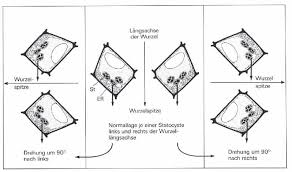
\includegraphics[width = 0.5\linewidth]{bilder/Graviperzeption.jpeg}
 	\caption{Statolithen und ER-Polster \label{Graviperzeption}}
 \end{figure} 

Dies ist aber nur der Fall bei Organen höherer Pflanzen, denn bei einer Einzelzelle, z.B einer \emph{Chara}-Rhizoide, erfolgt die Streckung nur durch Spitzenwachstum (einseitiges Wachstum der Zelle).
\emph{Dictyosomen} (flache, membranumhüllte Hohlräume in der Zelle) synthetisieren dabei Membran- und Zellwandbausteine unter dem Bereich der wachsenden Spitze und transportieren  die entstandenen \emph{Vesikel}.

Vesikel wandern auf der Oberseite, da beim Verlagern der Statolithen auf die Unterseite, der Weg dort damit gesperrt wird. Bei der Oberseite bewirken sie somit ein verstärktes Wandwachstum, also einen positiven Gravitropismus.

Bei gravitrop reagierenden Pilzen werden Amyloplasten durch {\glqq Glanzkörper\grqq} ersetzt, die die Funktion der Statolithen übernehmen, da Pilze keine Stärke enthalten. Diese in \emph{Vacuolen} liegenden Einschlusskörper besitzen einen hohes spezifisches Gewicht, da sie aus \ce{BaSO4} bestehen \parencite[453f]{Strasburger}.




\section{Signaltransduktion und differenzielles Wachstum}

\subsection{Teilnahme des Calciums bei der Signaltransduktion}

Die Signalübermittlung durch den direkten Kontakt zwischen Amyloplasten und ER wird als \emph{gravisensorische Transduktion} bezeichnet.
Durch den Druck der Amyloplasten auf die ER-Membranen wird ein \ce{Ca^{2+}}-Efflux (das Austreten von Molekülen oder Ionen an der Zellmembran) aus dem ER verursacht.
Dadurch wird die lokale \ce{Ca^{2+}}-Konzentration im  \emph{Cytoplasma} erhöht. 
Bereits ein Druck auf eine einzige ER-Zysterne reicht aus, um einen Efflux zu verursachen.

\subsection{Teilnahme des Elektronischen Feldes bei der Signaltransduktion}

Wichtiger bei der Signalumwandlung sind jedoch die Änderungen des elektrischen Feldes, dass die Wurzel umgibt.
Bei senkrecht stehenden Pflanzen wandern positive geladene Ionen (hier: Protonen) in die Wurzelspitze ein und treten im Bereich der Zellstreckzone wieder aus (?).

Diese Ionenbewegung wird als apoplastischer Strom bezeichnet, der das elektrisches Feld, das die Wurzel umgibt, erzeugt. Dieses Feld ist mit einer hochempfindlichen Vibrationselektrode nachweisbar. 
Wird die Pflanze horizontal gelegt, so werden die Wurzeln gravitropisch gereizt. Dabei gelangen die Protonen nur noch in die untere Flanke der Wurzelspitze hinein und auf der Oberseite hinaus (?), wodurch auch das elektrische Feld sich ändert \parencite[502f]{Nultsch}.



Dieses durch der Graviperzeption entstandene Signal kann nur in der Streckungszone hinter der Wurzelspitze aufgenommen werden. Kommt das Signal an, so setzt die Krümmung ein, indem die Flanken anfangen, ungleich zu wachsen. Damit ist feststellbar, dass der Perzeptions- und Reaktionsort getrennt sind.

Für diese Reaktion sind Präsentationszeiten des Reizes wichtig. Sie liegen meist zwischen 2 und 85 Minuten. Das dauert viel länger, als die kürzesten Reizeinwirkungen, die noch wahrgenommen werden können und unter 30 Sekunden liegen. (Kontrolle vllt gleicher text)
Somit wird bei jeder kleinen und kurzen Reizeinwirkung eine Vollführung der Krümmungsbewegung vermieden. Das ist wichtig für Pflanzen, um zum Beispiel eine gravitropische Reaktion auf eine Windeinwirkung zu verhindern \parencite[531]{Luettge}.


\subsection{Funktion der Auxine im Gravitropismus}

Die Ursache der Krümmung nach dem Signal ist die durch Schwerkraft hervorgerufene asymmetrische Verteilung des Auxins  \parencite[502f]{Nultsch}.

Auxin ist ein Pflanzenhormon, das viele Funktionen besitzt. Dabei ist die Stimulierung der Zellstreckung (nur in niedriger Konzentration) und die Seiten- und Adventivwurzelbildung (nicht aus einer apikalen (Sprossachse) oder einem basalen (Wurzel) Primärmeristem entstehend), besonders wichtig. 
Bei Pflanzen ist das natürliche Auxin die Indolessigsäure (IAA), aber alle Verbindungen, die zu einer Streckung von Koleoptilen führen, können als Auxin bezeichnet werden.
Andere Funktionen dieses Hormons wären die Regulierung der Fruchtentwicklung, Verstärkung der Apikaldominanz, Verzögerung der Blattfalls und Förderung der Leitgewebedifferenzierung.

Beim Krümmungsprozess wird Auxin von dee nur in eine Richtung direkt durch das  \emph{Parenchymgewebe} (Gewebe, dessen Zellen nebeneinander liegen) transportiert: Von der Sprossspitze längs der Sprossachse bis zur Basis(normal Satz machen). Dieser Transport wird als polarer Transport bezeichnet und ist nicht von der Schwerkraft abhängig.

Auxintransport geschieht durch Auxin-Transportproteinen, die sich am basalen Zellenende befinden, befinden.
Das Hormon wird zur Nachbarzelle am Apikalende transportiert.  durch diese Proteine hinausbefördert.

Auxine werden im Apikalmeristem der Sprossachse synthetisiert. Von dort aus bewegen sie sich zur Streckungszone und stimulieren dabei das Zellwachstum.
Jedoch ist diese Stimulierung nur dann möglich, wenn der Konzentrationsbereich des Auxins zwischen $10^{-8}$ bis $10^{-4}$ \si{\mole\per\L}. Bei höherer Konzentrationen kann Auxin die Zellstreckung durch Induktion der Ethylenbildung hemmen.

Bei der Wachstumsantwort der Zelle auf Auxin spielen Protonenpumpen eine entscheidende Rolle. Das Auxin stimuliert die Protonenpumpen der Plasmamembranen. Es werden Protonen herausgepumpt, wodurch eine Erhöhung des Membranpotenzials entsteht und der pH-Wert in der Zellwand gesenkt wird. 

Durch die Ansäuerung  der Zellwand werden Expansine, spezifische keilförmige Proteine, aktiviert, die die Zellwandstruktur auflockern, indem sie Wasserstoffbrückenbindungen zwischen Cellulosemikrofibrillen und anderen Zellwandbestandteilen lösen.

Das erhöhte Membranpotenzial führt zur erhöhten Ionenaufnahme in die Zelle und damit zur Erhöhung des osmotischen Drucks (\emph{Turgor}). Da die Zellwand plastisch ist, kann sich die Zelle nun ausdehnen. 

Auch die Genexpression wird von Auxin sehr stark beeinflusst, sodass neue Proteine von den Zellen in der Streckungszone gebildet werden.
Außerdem müssen Zellen mehr Cytoplasma und Zellwandmaterial bilden, da das Wachstum aufrecht erhalten werden muss. Dies wird auch durch Auxin stimuliert \parencite[1118ff]{campbell}.

Bei manchen Pflanzenarten (z.B. bei Sonnenblumen \emph{Helianthus} oder Bohnen \emph{Phaseolus}) spielt Auxin jedoch eine untergeordnete Rolle.
Die Steuerung der Krümmung dieser Pflanzenarten übernehmen Gibberelline \parencite[502f]{Nultsch}.
 
\subsection{Funktion der Gibberelline im Gravitropismus}

\emph{Gibberelline} sind, wie Auxin, Pflanzenhormone und besitzen mehrere Funktionen. 
Sie stimulieren die Sprossstreckung, beeinflussen Pollenentwicklung und sind für Pollenschlauch- und Fruchtwachstum sowie Samenentwicklung und Keimung verantwortlich. Außerdem bestimmen sie das Geschlecht in eingeschlechtigen Blüten und regulieren den Übergang von Jugendphasen zu Adultphasen. 
Bei der Zellstreckung wirken Gibberelline mit Auxin zusammen. Gibberelline aktivieren Enzyme, die die Zellwand auflockern und Expansinen (Proteine) den Eintritt in die Zellwand erleichtern \parencite[1122f]{campbell}.

 
Wie dargelegt, ist Gravitropismus ein lebenswichtiges Resultat eines komplexen und zum Teil noch unerforschten Zusammenspiels von biologischen Akteuren. Dennoch lässt sich die gesamte Kaskade mit einfachen Mitteln einleiten und kontrollieren, was zum experimentellen Teil der vorliegenden Arbeit führt. 



\chapter{Experimenteller Nachweis von Gravitropismus bei \emph{Lepidium sativum}}

\section{Methoden}

\subsection{Pflanzen}

Für das Experiment wurde die \emph{Lepidium sativum} (Kresse) genommen. Sie ist eine schnellwüchsige Pflanze und kann auf jedem lockeren, durchlässigen Gartenboden wachsen (der Firma Kiepenkerl).


\subsection{Verwendete Materialien und Geräte}

Außer den Pflanzen wurden vier gleich große Behälter und ein selbst gebautes Säckchen, eine Plastiktüte, ein Messzylinder (in ml) und Gegenstände für Stützung der Behälter (z.B. Holzklotz) verwendet.

Für die Pflanzen wurden Anzucht-Quelltabs (der Firma Windhager) benutzt, da die Erde torffrei ist und Kokosfasern enthält, die dafür sorgen, dass die Feuchtigkeit besser aufgenommen wird.

Dadurch können Samen schneller keimen und Wurzeln sich besser ausbilden, wodurch das Wachstum der Pflanze gefördert wird (http://www.windhager.eu/de/garten/anzucht/toepfe-quelltabs/anzucht-quelltabs-49892/). 

Für die Aufnahme des ganzen Experimentes wurde eine Kamera (Canon) verwendet.


\subsubsection{Klinostat}

create blueprint with OpenSCAD or LibreCAD or (paid) Autodesk

-(Bild?)

\subsection{Versuchsbeschreibung}

\subsubsection{Vorbereitung}

1. Tag (28.05.18): Aufbau des Experiments: alle Behälter mit der Anzuchterde gefüllt und auf der Plastiktüte (Vermeidung von Schmutz auf den Boden), Aussaat der Samen (jeweils 20 Stück in drei Behältern, gebliebene Samen in den vierten Becher (als Vergleichsergebnis gedacht), im Säckchen nur 3 Samen)

Bedingungen wie Zimmerlicht, Temperatur, Wasser (jeden Tag 20ml in jeden Behälter) werden eingehalten.

\subsubsection{Durchführung}

\begin{itemize}
	
\item 1. Tag (28.05.18): Aufbau des Experiments: alle Behälter mit der Anzuchterde gefüllt und auf der Plastiktüte (Vermeidung von Schmutz auf den Boden), Aussaat der Samen (jeweils 20 Stück in drei Behältern, gebliebene Samen in den vierten Becher (als Vergleichsergebnis gedacht), im Säckchen nur 3 Samen)
	  
\item 6. Tag (02.06.18): dabei Beginn des zweiten Experiments: verschiedene Positionierungen der drei Behälter: 1) vertikal zu Boden 2) Kopfüber 3) gewinkelt 
	
\item 7. Tag (03.06.18): neuer Versuch mit Klinostat: Start um 12:40, Ende am 9.Tag (05.06.18) um 23:45; 

\section{Ergebnisse}

\item 2. Tag (29.05.18): Keimung der Samen (Bild)

\item 3. Tag (30.05.18): Sprossen bis zu 2cm, noch keine Blätter, dennoch instabile Haft der Sprösslinge (noch nicht geeignet für das Experiment) 

\item 3. Tag (30.05.18): Sprossen bis zu 2cm, noch keine Blätter, dennoch instabile Haft der Sprösslinge (noch nicht geeignet für das Experiment)

\item 4. Tag (31.05.18): Gebildete Blätter, stabile Haft der Sprösslinge (geeignet für das Experiment), Säckchen bereit für den Versuch mit dem Klinostat (20 min für die Befestigung des Behälters an das Klinostat) und um 12.45 Versuch gestartet mit Geschwindigkeit 1 Umdrehung pro Minute;
um 15.45 gestoppt, da die Pflanzen sich vollständig gebogen haben (nach außen die Sprossen, nach innen die Wurzeln), Foto 1 und 2

\item 5. Tag (01.06.18): Über Abend Rückbildung der Pflanzen, gleicher Versuch nochmal möglich, diesmal mit genauen Zeitangaben; aber um 12:53 (des nächsten Tages) Klinostat kaputt gefunden; Pflanzen haben aber angefangen sich sichtbar zu biegen (gelaufene Zeit ca. 1 Stunde und 8 Minuten)

\item 6. Tag (02.06.18): Klinostat wieder repariert (mit Uhu-Kleber), Sprossen fast bis zu 3cm

\item 7. Tag (03.06.18): Bemerkung: Sprossen über 3cm (Annahme, dass die Krümmung deshalb verlangsamt war); Foto 5 (kleinerer Spross gebogen, größerer Spross nur geneigt)

\item Krümmung sichtbar auch bei dem zweiten Versuch (-zwei Bilder)

\end{itemize}

\section{Diskussion}

\chapter{Fazit und Ausblick}


\printbibliography

% afa
% \begin{figure}
% 	\centering
% 	\includegraphics[width = .5\linewidth]{images/IMG_1117.JPG}
% 	\caption{a nice little caption \label{nice_picture}}
% \end{figure}
% asd
% a
% 
% as we see in image \ref{nice_picture}
% 
% \begin{figure}
%  \centuring 
%  \includegraphics [width = .5\linewidth]{images/IMG_1083.JPG}
%  \end {figure} 
% Photo 1
%
% \begin{figure}
%  \centuring 
%  \includegraphics [width = .5\linewidth]{images/IMG_1073.JPG}
%  \end {figure} 
% Photo 2

%\begin{figure}
	%  \centuring 
	%  \includegraphics [width =.5\linewidth]{images/IMG_1399.JPG}
	%  \end {figure} 
	% Photo 5

http://www.digitalefolien.de/biologie/pflanzen/aufbau/zell.html (Pflanzenzelle)

https://www.lernhelfer.de/schuelerlexikon/biologie/artikel/wurzel (Wurzelabschnitt)

https://www.lernhelfer.de/schuelerlexikon/biologie/artikel/wurzel (Wurzelabschnitt2)

https://www.lernhelfer.de/schuelerlexikon/biologie-abitur/artikel/bau-und-funktion-der-wurzel (Wurzelabschnitt3)

http://www.plantphysiol.org/content/120/2/343 (Statolithen2)

Bild-Differenzielles Wachstum (selbstgemachtes diff.png)

http://www.zum.de/Faecher/Materialien/beck/12/bs12-2.htm (Pflanzenaufbau)
\end{document}
